\documentclass[logo,reportComp]{thesis}
\usepackage[python,pseudo,linenum]{mypackage}
\usepackage{pythonhighlight}

\title{机器学习与数据挖掘大作业}
\subtitle{多标签用户人格分类(集成学习)}
\school{数据科学与计算机学院}
\author{陈鸿峥}
\classname{17大数据与人工智能}
\stunum{17341015}
\headercontext{机器学习与数据挖掘大作业}

\let\emph\relax % there's no \RedeclareTextFontCommand
\DeclareTextFontCommand{\emph}{\kaiti\em}

\begin{document}

\maketitle
\tableofcontents

\newpage
\section{题目描述}
MBTI理论认为一个人的个性可以从四个角度进行分析,用字母代表如下:
\begin{itemize}
    \item 驱动力的来源:外向E---内向I
    \item 接受信息的方式:感觉S---直觉N
    \item 决策的方式:思维T---情感F
    \item 对待不确定性的态度:判断J---知觉P
\end{itemize}
按照不同的组合,可以产生16种人格类型。

本次大作业要求利用机器学习方法,通过用户的发言记录对用户的人格类型进行分类\footnote{数据集链接:\url{https://www.kaggle.com/datasnaek/mbti-type}}。

本实验报告为大作业的第一部分---\textbf{集成学习}方法。

\section{预处理}
由于原始数据集为用户在网页上的发言记录,非常随意及杂乱,故做分类任务前的第一步需要灵活应用上学期自然语言处理学过的知识,对数据集进行预处理操作。
主要分为文本清洗、词典生成、词向量生成三个步骤。

\subsection{文本清洗}
文本清洗一步依序进行了以下操作。
\begin{enumerate}
	\item 标点后强制添加空格。
	由于是网页发言记录,很多用户可能不会太过在意标点符号后面是否有空格。如果没有添加,则之后删除标点可能会导致前后两个词语粘连。
	\item 移除网页链接。
	由于网页地址通常没有太多含义,故这里直接将发言记录中出现的网页链接直接移除。
	采用以下的正则表达式对http/https开头的网址进行匹配。
\begin{lstlisting}
(http|https):\/\/.*?( |'|\")
\end{lstlisting}
	\item 移除数字。
	同理,数字带来的信息非常少,无法作为区分人格的合理因素,故也将其移除。
	\item 移除标点符号。
	我们做文本分类时,关心的是用户说过的词语,而不是他是否有进行断句,故也将所有标点符号移除。
	这里采用了一种比较高效的方法,直接调用C库对字符串进行处理。
\begin{lstlisting}
new_post = new_post.translate(str.maketrans('', '', string.punctuation))
\end{lstlisting}
	注意两条评论之间采用\verb'|||'进行分隔,但我们直接将其移除了,意味着我们并不关心用户发言记录的先后顺序,我们更关心的其说过什么话。
	\item 移除空格。
	句子内部空格用正则表达式匹配\verb'" +"'后用单一空格代替;句子前后的空格用Python内置的\verb'strip'函数即可移除。
	\item 字母小写化。
	避免计算机认为不同大小写字母构成的为不同的词语,如"Hello"和"hello"两者意思相同,代表的是同一个词,故要进行规范化。
	\item 移除停止词(stopping words)。
	这是很多NLP任务中必备的一步,因为停止词并不会带来任何更多语义上的信息。
	这里采用上学期NLP大作业提供的停止词列表\cite{bib:stopping_words}。
\end{enumerate}

做完上述预处理后,即可将处理后的用户发言存成文档/列表,文档中的每一行或列表中的每一项即为对应用户所说过的所有词语。

这里做的操作都比较常规,并没有对该数据集进行特定优化,如果后续作业中想继续对预处理部分进行改进,可以考虑以下几个方面:
\begin{itemize}
	\item 表情符号的处理。
	从这些用户的发言记录中可以发现,外国网友也是很喜欢用emoji甚至颜文字的。
	emoji比较好辨别,均用两个冒号括起来,如\verb':sad:'。
	颜文字如\verb':)'和\verb':(',这是用得比较多的,但被我们在前面的预处理中移除了。
	而喜欢用这些表情符号的可能恰恰对应着某一类人,因此可以单独对其进行处理,做成单独的特征,供后续的机器学习模型使用。
	\item 词型变位。
	目前还没有做这方面的处理,可能需要结合nltk包将不同的词性但代表同一个词语的单词进行合并。
	这可能会对后续词频及词向量的生成造成一定影响。
\end{itemize}

\subsection{生成词典}
由于机器学习任务通常都是输入数字值,因此需要将单词全部转为数字标号,以便之后更好送入机器学习模型。

主要的操作有以下几步:
\begin{enumerate}
	\item 构造词表。
	将所有用户所说过的词语合并起来即构成词表。
	\item 词频计数。
	将Python标准库中的\verb'Counter'作用在词表上,即可得到每个词语的词频。
	\item 添加未知词标记。
	NLP任务中常常有未登录词(Out-of-vocabulary, OOV)的情况出现,即在测试集中出现的词语可能并未在训练集中出现。
	因此需要添加\verb'<UNK>'标记,并将其标号为$0$,以更好处理这种情况。
	(之后采用更强大的机器学习模型,可能还需要对句子进行对齐处理,这时还需要添加\verb'<PAD>'标记)
	\item 删除词频过小的词语。
	词频过小的词语对预测任务并没有带来太多实质性的帮助,同时还会导致特征空间维度过大,因此需要提前将这些词语给删除。
	\item 依词频排序。
	对遗留的词语依照词频降序排序。
	\item 基于词频生成词嵌入。
	通过读取排序的序号,即可生成词语到数字标号的双向映射。
\end{enumerate}

完整过程如下面程序所示。
\lstinputlisting[firstline=102,lastline=115]{../Ensemble.py}

\subsection{生成词向量}
由于第一次任务较为简单,故这里直接使用词袋模型(Bag of Words, BoW)\cite{bib:bow}构造词向量。

考虑词典中所有词语为$\{w_i\}_{i=1}^M$,其中$M$为词典大小。
那么对于每一用户$uid$的发言,可构造词向量
\[\vv_{uid}=\bmat{\sW_{uid}(w_1) & \sW_{uid}(w_2) & \cdots & \sW_{uid}(w_M)}^\T\]
其中$\sW_{uid}(w_i)$计算用户$uid$中$w_i$出现的次数。
这里同样可以直接通过Python标准库的\verb'Counter'类进行计数。
注意这里需要利用前面构造的词典将字符串单词转换为数字标号,如果词典中该词没有出现,则标号为$0$\verb'<UNK>'。

最终构造出来的词袋模型(也即送入机器学习模型的特征)为$N\times M$大小的矩阵,其中$N$为用户数目。

\section{集成模型}
下面将介绍构造集成模型并进行训练预测的完整过程。
这里我采用了随机森林作为集成模型,基学习器为决策树。

\subsection{决策树}
在本次实验中,我自己实现了ID3决策树,以信息增益作为决策准测,并添加了预剪枝的机制。

\subsubsection{熵与信息增益}
依据信息熵的定义,假定当前样本集合$D$中第$k$类样本所占的比例为$p_k(k=1,2,\ldots,|\mathcal{Y}|)$,则$D$的信息熵为
\[\mathrm{Ent}(D)=-\sum_{k=1}^{|\mathcal{Y}|}p_k\log_2 p_k\]

又假定离散属性$a$有$V$个可能的取值$\{a^1,a^2,\ldots,a^V\}$,若使用$a$来对样本集$D$进行划分,则会产生$V$个分支结点,其中第$v$个分支结点包含了$D$中所有在属性$a$上取值为$a^v$的样本,记为$D^v$,进而可计算出信息增益
\[\mathrm{Gain}(D,a)=\mathrm{Ent}(D)-\sum_{v=1}^V\frac{|D^v|}{|D|}\mathrm{Ent}(D^v)\]

为了高效实现信息熵和信息增益的计算,我并没有采用Python的裸循环实现,而是利用NumPy的向量化计算方法。
对照上述公式实现可得到以下代码。
\lstinputlisting[firstline=228,lastline=253]{../Ensemble.py}

\subsubsection{树结点}
决策树最基本的单元即树的结点,这里我采用一个\verb'Node'类进行封装。
其中可以设置是叶子(leaf)结点还是分支(branch)结点,并用字典存储其孩子对象,方便后续的访问及遍历。
\lstinputlisting[firstline=258,lastline=280]{../Ensemble.py}

\subsubsection{树构造}
依照西瓜书中给出的决策树算法,可以对应写出\verb'TreeGenerate'函数。
\begin{figure}[H]
\centering
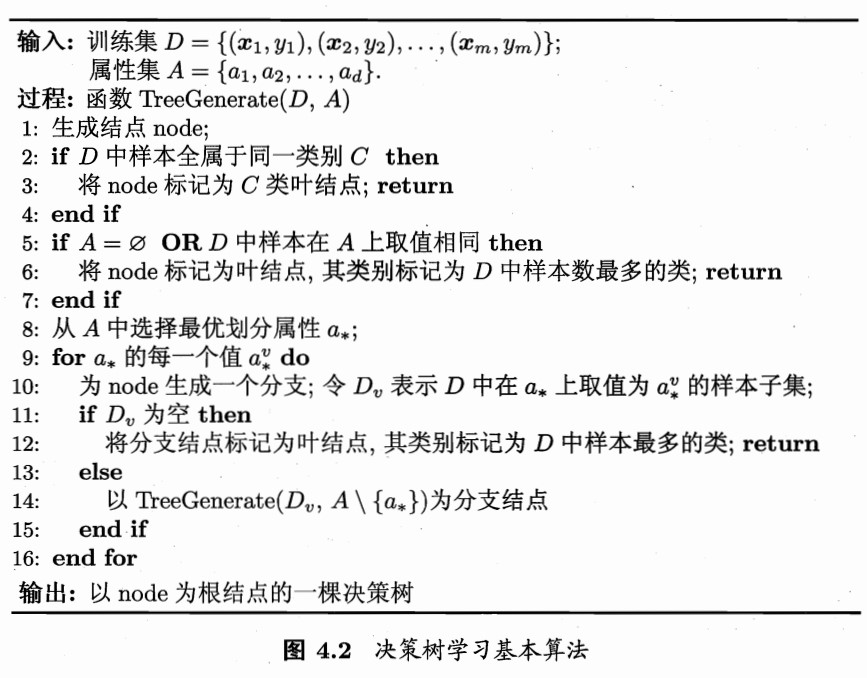
\includegraphics[width=0.8\linewidth]{fig/dt_pseudo.jpg}
\end{figure}

下列代码中已经将上述的三种情况全部标注出来,详情见代码中的注释。
为了提升泛化能力,这里还提供了预剪枝(pre-pruning)机制。
\lstinputlisting[firstline=308,lastline=396]{../Ensemble.py}

从代码中可以看到,对特征数据的处理都尽可能采用NumPy的向量化方式,及fancy indexing进行索引,这样能够最大程度提升性能,避免不必要的解释运行开销。

另外,在代码第24行引入了随机化特征选择,这会在下面的部分进行叙述。

\subsection{随机森林}
随机森林如算法\ref{alg:rf}所示。
这里有几个关键点:
\begin{itemize}
	\item 在决策树特征选取过程中引入随机化因素。
	原来的决策树是在当前结点的所有属性值中挑选最优的一个,现在则是从当前结点所有属性值中先挑选$k$个,再从这$k$个中选择最优的一个。
	这里$k$取$\lfloor\log_2 d\rfloor+1$,其中$d$为属性数目。
	\item 采用自助采样法(bootstrap sampling)对输入的训练集进行选择,同样是提升泛化能力的有效机制。
	\item 最终利用bagging的方式进行预测,具体实现中采用了简单投票法。
\end{itemize}
\begin{algorithm}
\caption{Random Forest (Bagging)}
\label{alg:rf}
\begin{algorithmic}[1]
\For{$t=1,2,\ldots,T$}
\State Use bootstrap sampling to generate $\mathcal{D}_{bs}$
\State $h_t=RF(\mathcal{D}_{bs})$
\EndFor
\State \Return $\displaystyle H(\vx)=\argmax_{y\in\mathcal{Y}}\sum_{t=1}^T\vone(h_t(\vx)=y)$
\end{algorithmic}
\end{algorithm}

完整的随机森林构造如下所示,这里参照了sklearn的API函数签名以方便后续实验对比,但里面的代码均为自己实现。
\lstinputlisting[firstline=457,lastline=503]{../Ensemble.py}

注意这里还使用了Python的多进程库\verb'multiprocessing'\footnote{之所以不使用多线程是因为Python具有全局解释器锁(Global Interpreter Lock, GIL),在多线程执行过程中会造成非常大的性能损耗。}来进行并行计算。
由于每棵决策树的构造过程都是独立的,因此对每棵树分配一个进程即可。
进程与进程之间直接采用文件进行通信。

\subsection{模型训练与预测}
有了上述封装好的模块,要进行模型训练与预测就比较容易了,如下调用函数。
\lstinputlisting[firstline=509,lastline=512]{../Ensemble.py}

\subsection{其他实现细节}
\begin{itemize}
\item 只使用了基本了numpy和pandas库用于做矩阵运算及数据处理,引入sklearn库仅用于数据集划分及实验对比。
\item 预处理的中间结果用NumPy或pickle文件保存。重新执行时会先判断文件是否存在,如果存在则直接读取,而不用重复进行预处理。
\end{itemize}

\section{实验结果}
本次实验的完整代码可见附件中的\verb'Ensemble.ipynb'或由Jupyter Notebook生成的\verb'Ensemble.py'文件。

\subsection{超参数选择}
实验所采用的超参数如表\ref{tab:hyperparam}所示。
之所以要设置词典最小词频和决策树最大深度,是为了减少特征维度,进而缩短训练时间。
\begin{table}[H]
\caption{超参数设置}
\label{tab:hyperparam}
\centering
\begin{tabular}{|c|c|}\hline
词典中的最小词频 & 5 \\\hline
随机森林基学习器数目 & 1,3,5,10\\\hline
决策树最大深度 & 10\\\hline
训练集测试集比例 & 7:3\\\hline
\end{tabular}
\end{table}

生成的特征矩阵维度为$8676\times 27129$,前者为用户数目,后者为词典大小。

\subsection{综合比较}
最终各类别的F1及精确度指标如图\ref{fig:f1}所示,可以看到我的随机森林最终达到了31\%的准确率。
\begin{figure}[H]
\centering
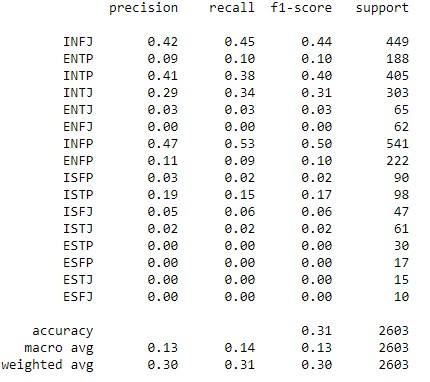
\includegraphics[width=0.8\linewidth]{fig/report.jpg}
\caption{实验结果}
\label{fig:f1}
\end{figure}

从图中可以看出能够预测准确的基本上都是出现次数比较多的,而对于出现较少的性格基本预测不出。
这其实很大程度是因为原始数据集各类别的分布不均,如图\ref{fig:distribution}所示。
该数据集中ESTJ、ESFJ、ESFP等性格出现的次数本来就少,要从仅仅几十个样本中就学出其规律,对于人类来说都很难,更何况是机器,故可以看到这些类别的F1分数均为0。
如果要处理好这种情况,则可能会涉及到小样本学习(few-shot learning)。
这已经超出了本次实验的范围,故在此不做更加深入的分析。
\begin{figure}[H]
\centering
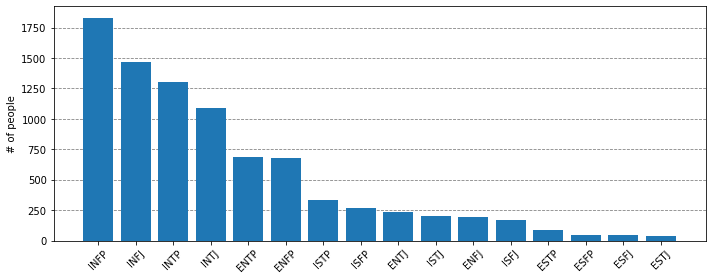
\includegraphics[width=\linewidth]{fig/distribution.png}
\caption{用户个性分布}
\label{fig:distribution}
\end{figure}

为了探究不同超参数对模型的影响,我也比较了我自己实现的随机森林与sklearn默认随机森林的结果,如图\ref{fig:hyper}所示。
可以看到单棵决策树我的性能要比sklearn的性能高几个百分点,但随着决策树数目的增加,sklearn的效果越来越好,并超过我的随机森林的性能。
这很大程度取决于自助采样的选择以及超参数随机化因子的设定。
同时由于没有在决策树内部开启并行计算,我实现的版本比sklearn的版本要慢上几个数量级。
\begin{figure}[H]
\centering
\begin{tabular}{cc}
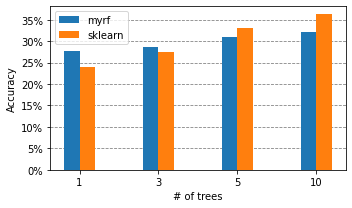
\includegraphics[width=0.5\linewidth]{fig/accuracy.png}&
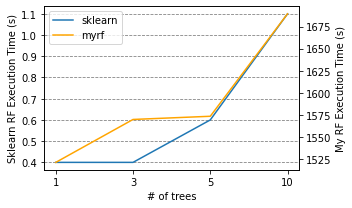
\includegraphics[width=0.5\linewidth]{fig/exe_time.png}
\end{tabular}
\caption{不同超参数下准确率与运行时间比较}
\label{fig:hyper}
\end{figure}

但总的来说,我的精度与sklearn的精度控制在合理的范围内,并且对于该数据集表现出了较好的泛化能力。

\section{总结与思考}
本次实验相对来讲比较简单,对于文本数据充分利用上学期自然语言处理课程的知识来进行处理,而难点应该是在后面的手写决策树及随机森林。
由于有一定的代码量,因此这一部分还是调试了挺长时间。
为了验证决策树的正确性,还先利用西瓜书里面的数据集进行测试。
确保没有问题后,才将其运用到此次Kaggle的数据集中。

此次实验还有很多未完善的地方,如未做特征工程(利用PCA等工具先进行降维),未采用更好的词向量模型(如TF-IDF和word2vec),未对样本量较少的类别进行处理等,这些都可以在之后的实验中继续进行补充。
另外从本次实验中也可以看出NLP相关任务的难度,即使是采用了强大的机器学习模型,但预测准确率依然比较低,不过这也给了之后的实验更大的探索空间。

\begin{thebibliography}{99}
\bibitem{bib:stopping_words} Stopwords, \url{https://github.com/goto456/stopwords}
\bibitem{bib:bow} Bag of words model, \url{https://en.wikipedia.org/wiki/Bag-of-words_model}
\end{thebibliography}

\end{document}

% 作业内容:
% 1. 使用集成学习方法完成人格分类(6月10日)
% * 对数据进行预处理
% * 使用集成学习模型(AdaBoost或Random Forest)进行人格分类
% * 提交报告及代码
% 2. 使用SVM进行人格分类(6月30日)
% * 数据预处理
% * 使用SVM进行人格分类
% * 提交报告及代码
% 3. 使用深度学习模型进行人格分类(7月31日)
% * 数据预处理
% * 使用深度学习模型(不限)进行人格分类
% * 提交代码和报告
% ** 深度学习方法需要有方法上的创新,如果只简单使用开源代码或框架,最多只能拿8分
% ** 加分项:使用英文撰写报告,设计合理实验(对比不同模型表现/不同超参数对性能的影响),自己撰写模型代码,尽可能少调用工具

% 评价指标:
% * 单独对每种类别进行评价/整体评价
% * F1 \& Accuracy

% 评分:
% * 集成学习方法:8分
% * SVM方法:8分
% * 深度学习方法:14分